\documentclass{beamer}
\usepackage{verbatim}
\setlength{\parindent}{0em}
\setlength{\parskip}{0.5em}
\usepackage{graphicx}
%\usepackage{mdwlist}
\usepackage[mathscr]{euscript}
%\usepackage{amssymb}
\setbeamertemplate{itemize item}[circle]
\setbeamertemplate{itemize subitem}[square]
\definecolor{mine}{RGB}{155,155,155}
\definecolor{fpink}{rgb}{0.99, 0.56, 0.67}
\definecolor{oj}{rgb}{1.0,0.65,0.0}
\definecolor{cblue}{rgb}{0.39, 0.58, 0.93}
\definecolor{turq}{rgb}{0.0, 0.81, 0.82}
\definecolor{cgreen}{rgb}{0.0, 0.8, 0.6}
\definecolor{lemon}{rgb}{1.0, 0.97, 0.0}
\definecolor{pur}{rgb}{0.88,0.69,1.0}
\definecolor{cpink}{rgb}{0.92, 0.3, 0.26}
\definecolor{mangotango}{rgb}{1.0,0.51,0.26}
\setlength{\unitlength}{1mm}

\setbeamercolor{normal text}{bg=black, fg=white}
\setbeamercolor{title}{fg=cgreen}
\setbeamercolor{frametitle}{fg=cgreen}
\setbeamercolor{framesubtitle}{fg=cblue}
%\setbeamercolor{block title}{fg=green}
\setbeamercolor{itemize item}{fg=cpink}
\setbeamercolor{itemize subitem}{fg=pur}
\setbeamercolor{enumerate item}{fg=cpink}

\usefonttheme{serif}
\setbeamerfont{framesubtitle}{size=\large}
\setbeamerfont{frametitle}{series=\bfseries}
%\usepackage{fontspec}
%\setmainfont{}

\begin{document}

\begin{frame}
    \begin{centering}
    {\Large Basic Principles of Solar Acoustic Holography}
    {\large\textcolor{cblue}{Laurel Farris}}\\
    {\large\textcolor{cblue}{ASTR 500}}\\
    {\textcolor{cblue}{11 March 2016}}\\
    \end{centering}
    \vspace{1cm}
    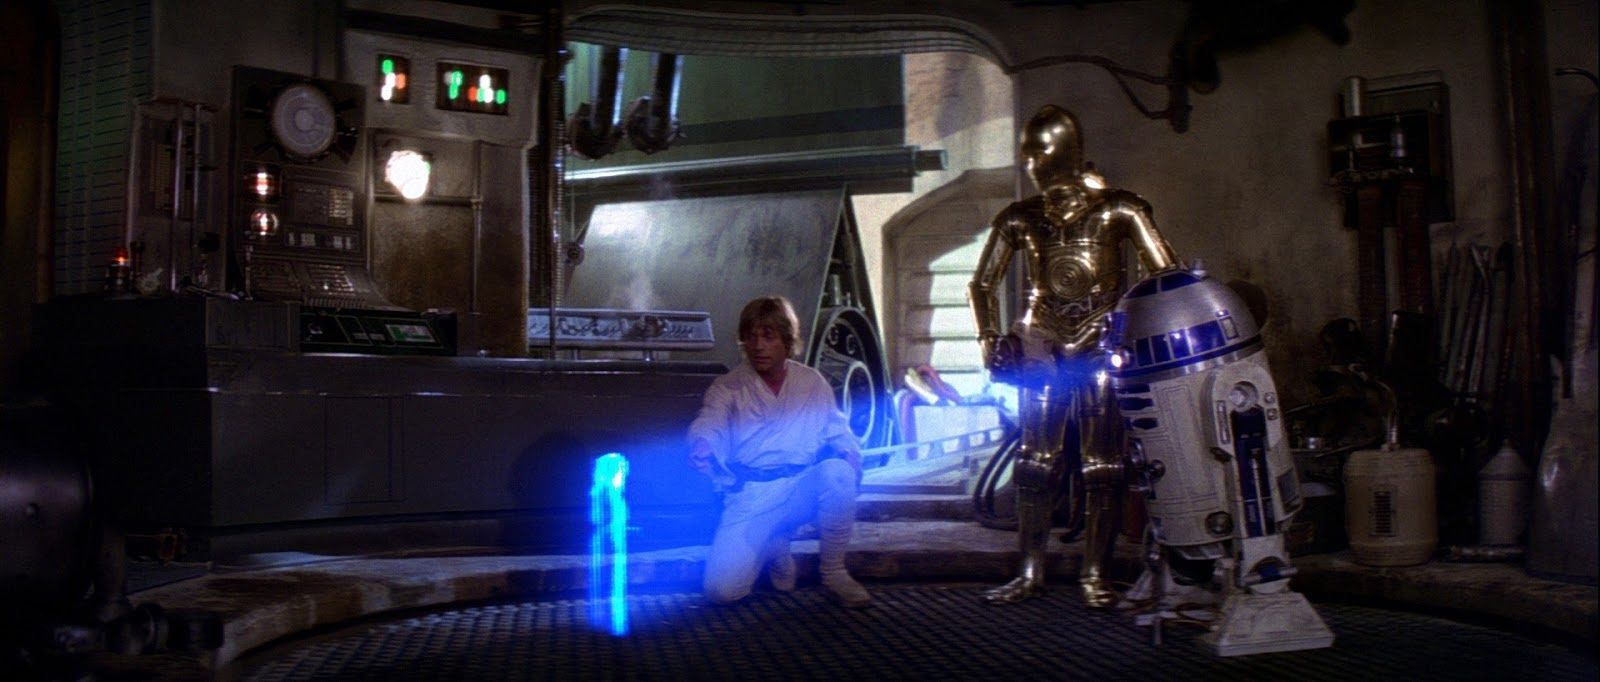
\includegraphics[width=\paperwidth]{starwars.jpg}
\end{frame}

\begin{comment}
\begin{frame}{Outline}
    \begin{enumerate}
        \item Basic principles of helioseismic holography
        \item Historical stuff
        \item Simple acoustic power holography
        \item Phase-sensitive holography
        \item Examples of applications
    \end{enumerate}
\end{frame}
\end{comment}
%----------------------------------------------------------------%
\begin{frame}{Heliospheric Holography}
What is it?
\begin{itemize}
    \item \large\textcolor{mangotango}{Computational seismic
        holography is accomplished by the \emph{phase-coherent}
        wave-mechanical reconstruction of the \emph{p}-mode
        acoustic field into the solar interior based on helioseismic
        observations at the solar surface}
        \normalsize
        \begin{enumerate}
            \item Observe disturbance on surface
            \item Reverse time to identify source
        \end{enumerate}
\end{itemize}
Why use it?
\begin{itemize}
    \item Space-weather forecasting:\\
    predict flares before they face Earth!
\end{itemize}
\end{frame}
%----------------------------------------------------------------%
\begin{frame}{Comparison with optics}
    \begin{itemize}
        \item Submerged sources in sun $\sim$ things we see
        \item Photosphere $\sim$ surface of cornea (front of eye)
    \end{itemize}
    Both involve refocusing radiation to render stigmatic images
    that can be sampled over focal surface at any desired depth.
    \begin{figure}
        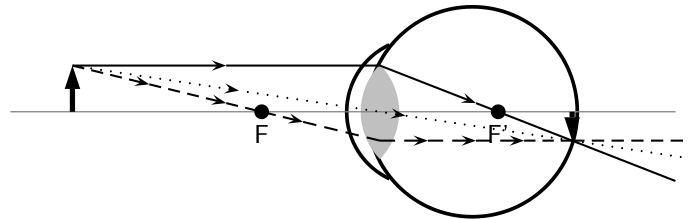
\includegraphics[width=\textwidth]{eye.png}
    \end{figure}
\end{frame}
%----------------------------------------------------------------%
\begin{frame}{Historical Note}
    \begin{itemize}
        \item Concept proposed in 1975 by Roddier
        \item Developed over the 1990s by Lindsey and Braun\\
            $\rightarrow$ Key to locating and examining
            fine structure in the interior and far side of the sun.
    \end{itemize}
    Seismic holography was first applied to helioseismic data from
    the SOlar Heliospheric Observatory (SOHO).\\
    ``New'' (1998 - 1999) solar acoustic phenomena:
    \begin{itemize}
        \item `acoustic moats' surrounding sunspots
        \item `acoustic condensations' 10\-20 Mm beneath active regions
        \item `acoustic glories' surrounding complex active regions
        \item first helioseismic images of a flare
    \end{itemize}
\end{frame}
%----------------------------------------------------------------%
\begin{frame}
    \Large
    \textcolor{lemon}{``Heismic holography should \emph{not} be
    indentified as a method for physical \emph{modelling} of solar
    interior structure.''}
\end{frame}
%----------------------------------------------------------------%
\begin{frame}{``Basic Principles of Solar Acoustic Holography''}
    {C. Lindsey and D. C. Braun (2000)}
    \begin{itemize}
        \item Compare simple acoustic-power to phase-sensitive
        \item Propose ``simple computational principles'' to produce images
            from high quality helioseismic observations.
    \end{itemize}
\end{frame}
%----------------------------------------------------------------%
\begin{frame}{Step 1: Helioseismic observations}
    \begin{figure}
        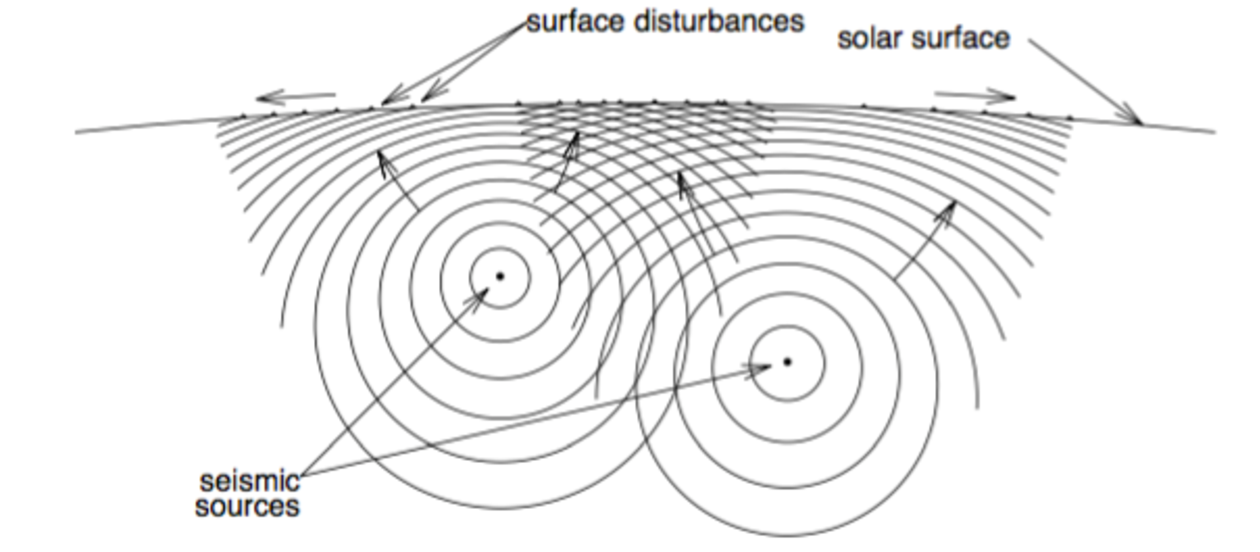
\includegraphics[width=\textwidth]{fig_1.pdf}
    \end{figure}
    \begin{itemize}
        \item Acoustic waves are produced in the interior
        and travel \emph{upward}.
        \item Pattern of ripples appears on surface
            directly \emph{above} the sources (what we observe).
        \item The waves are \emph{absorbed} upon reaching the surface.
    \end{itemize}
\end{frame}
%----------------------------------------------------------------%
\begin{frame}{Step 2: Apply observations to a model}
    \begin{figure}
        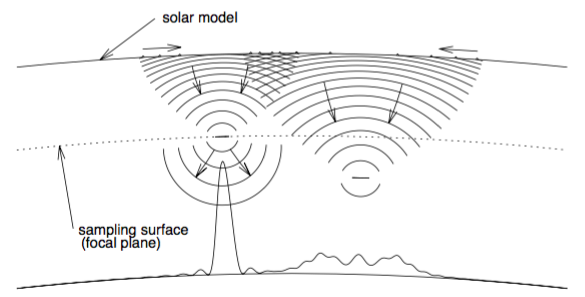
\includegraphics[width=\textwidth]{fig_2.png}
    \end{figure}
    \begin{itemize}
        \item Disturbance now propagating back down.
        \item ``Focal plane'' lies in the interior, at a depth
            $z_{\textrm{plane}}$.
    \begin{itemize}
        \item $z_{\textrm{plane}} = z_{\textrm{source}}$:
            diffraction-limited signature
        \item $z_{\textrm{plane}} \neq z_{\textrm{source}}$:
            unfocused, diffuse profile
    \end{itemize}
    \end{itemize}
\end{frame}
%----------------------------------------------------------------%
\begin{frame}{3-D perspective}
    \begin{figure}
        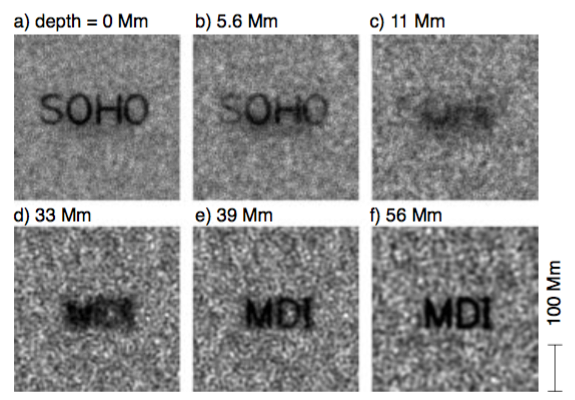
\includegraphics[width=0.9\textwidth]{fig_3.png}
    \end{figure}
    \vspace{-0.5cm}
    \begin{columns}
        \column{0.5\paperwidth}
            \begin{itemize}
                \item $z_{\textrm{SOHO}} = 0$ Mm
                \item $z_{\textrm{MDI}} = 56$ Mm
                    ($\sim \frac{1}{10}$ R$_{\odot}$).
            \end{itemize}
        \column{0.5\paperwidth}
            \begin{itemize}
                \item (b) \& (c) acoustic \emph{stalactites}
                \item (d) \& (e) acoustic \emph{stalagmites}
            \end{itemize}
    \end{columns}
\end{frame}
%----------------------------------------------------------------%
\begin{frame}
\Large\textcolor{lemon}{Seismic holography is \emph{not} in any sense
a representation or approximation of solar acoustics in terms of ray
optics.}
\end{frame}
%-------------------------------------------------------------------%
\begin{frame}{The Computational Task}
    Two perspectives:
    \begin{enumerate}
        \item ``spectral''
            \begin{itemize}
                \item wavenumber-frequency $(k,\nu)$
                \item (computationally advantageous)
            \end{itemize}
        \item ``time distance''
            \begin{itemize}
                \item space-time $(x,t)$
                \item (more intuitive)
            \end{itemize}
    \end{enumerate}
Can extrapolate the (incomplete) acoustic field in the interior.
\end{frame}

\begin{comment}
\begin{frame}{The Computational Task}
    Two perspectives:
    \begin{enumerate}
        \item ``spectral''
            \begin{itemize}
                \item wavenumber-frequency $(k,\nu)$
                \item (computationally advantageous)
            \end{itemize}
        \item ``time distance''
            \begin{itemize}
                \item space-time $(x,t)$
                \item (more intuitive)
            \end{itemize}
    \end{enumerate}
    Given
    \begin{itemize}
        \item acoustic amplitude
        \item derivative normal to surface surrounding medium that is
            free of sources, sinks, or scatterers
    \end{itemize}
    can extrapolate the (incomplete) acoustic field in the interior.
\end{frame}
\end{comment}

\begin{frame}{The space-time perspective}{Acoustic \emph{egression}}
    \begin{itemize}
        \item $\psi(\mathbf{r}',t')$: \emph{Actual} acoustic field
        \item $H_{+}(\mathbf{r},z,t)$:
            \emph{incomplete regression} of the acoustic field
        \item $(\mathbf{r}',0,t')$ $\rightarrow$ surface
        \item $(\mathbf{r},z,t)$ $\rightarrow$ focal point
    \end{itemize}
    $$ H_{+}(\mathbf{r},z,t) = \int
    \textrm{d}t' \int\limits_{a<|\mathbf{r}-\mathbf{r}'|<b}
    \textrm{d}^{2}r'G_{+}
    (|\mathbf{r}-\mathbf{r}'|,z,t-t')\psi(\mathbf{r}',t')  $$
    \textcolor{lemon}{$$ H_{+} = G_{+} * \psi{'} $$}
    \textcolor{pur}{$G_{+}$} $\rightarrow$
    Green's function that expresses how a single transient point
    disturbance propagates forward or backward in time between
    $(\mathbf{r}',0,t')$ and $(\mathbf{r},z,t)$.

\end{frame}

\begin{frame}{The space-time perspective}{Acoustic \emph{ingression}}
    $H_{-}$: ``acoustic ingression'', the time reversal
    of $H_{+}$; waves converge into the focal point
    and contribute to the disturbance.

    Green's function:
    $$ G_{-}(|\mathbf{r}-\mathbf{r'}|,z,t-t') =
    G_{+}(|\mathbf{r}-\mathbf{r'}|,z,t'-t) $$
\end{frame}
%-------------------------------------------------------------------%
\begin{frame}{The wavenumber-frequency perspective}
    \begin{itemize}
        \item $\hat{\psi}(\mathbf{k},\nu)$: Fourier transform of $\psi(\mathbf{r},t)$
        \item $\hat{G}_{+}(|\mathbf{k}|,z,\nu)$: Fourier transform of
            $G_{+}(|\mathbf{r}|,z,t)$
    \end{itemize}
    From the convolution theorem:
    $$ \hat{H}_{+}(\mathbf{k},z,\nu) = \hat{G}_{+}(|\mathbf{k}|,z,\nu)
     \hat{\psi}(\mathbf{k},\nu) $$
    \textcolor{lemon}{$$ \hat{H}_{+} = \hat{G}_{+} \times \hat{\psi}{'} $$}
     Multiplication is computationally \emph{faster} than convolution,
     so this is the preferred method.
\end{frame}
%-------------------------------------------------------------------%
    %After computing $H_{+}$, square and integrate it to produce an egression
    %power map over the time period in desired range.
\begin{frame}{Temporal Fourier Transform}
    Need large pupils to image deeper focal planes,
    but this produces coma, primary astigmatism, and higher-order aberrations.
    $$(\mathbf{r},t) \rightarrow (\mathbf{r},\nu)$$\\
    $$ \check{H}_{+}(\mathbf{r},z,\nu) =
    \int\limits_{a<|\mathbf{r}-\mathbf{r}'|<b}\textrm{d}^{2}r'\check{G}_{+}
        (|\mathbf{r}-\mathbf{r}'|,z,\nu)\check{\psi}(\mathbf{r}',\nu) $$
    \textcolor{lemon}{$$ \check{H}_{+} = \check{G}_{+} * \check{\psi}{'} $$}
\end{frame}
%-------------------------------------------------------------------%
\begin{frame}{Subjacent vs. Superjacent Vantage Holography}

    {\large\textcolor{cblue}{\textbf{Superjacent:}}}
    \begin{itemize}
        \item Wave propagated directly \emph{upward} from the source
            to surface
        \item applies to active regions.
    \end{itemize}
    {\large\textcolor{cblue}{\textbf{Subjacent:}}}
    \begin{itemize}
        \item inner radius, $a$, of the pupil annulus is much greater than
            the depth of the focal plane;
        \item applies to quiet sun (often the practical choice)
    \end{itemize}
\end{frame}
%-------------------------------------------------------------------%
\begin{frame}{Subjacent Vantage Holography}
    \begin{figure}
        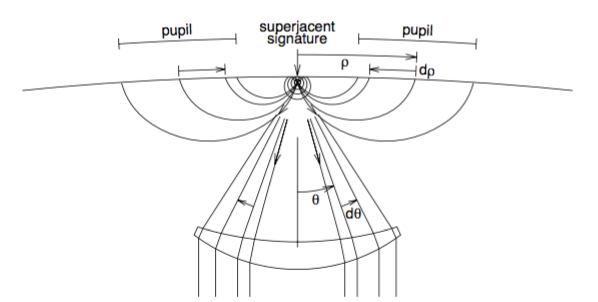
\includegraphics[width=\textwidth]{fig_4.png}
    \end{figure}
\end{frame}
%-------------------------------------------------------------------%
\begin{frame}
    \begin{figure}
        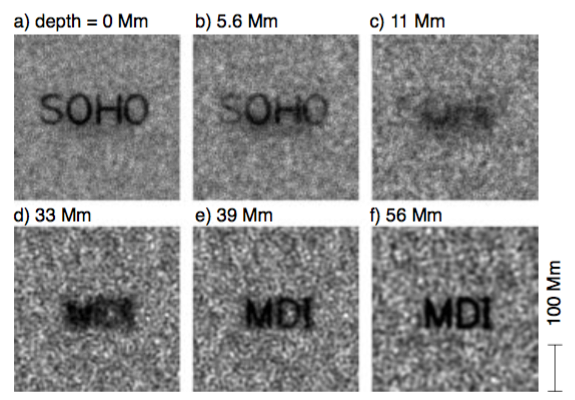
\includegraphics[width=0.9\textwidth]{fig_3.png}
    \end{figure}
    \vspace{-0.25cm}
    \begin{itemize}
        \item $a$ = 15 Mm, $b$ = 45 Mm
        \item (a) \& (b): superjacent
        \item (c) mixed perspective
        \item (d), (e), \& (f): predominantly subjacent
    \end{itemize}
\end{frame}
%-------------------------------------------------------------------%
\begin{comment}
\begin{frame}{A word about diffraction limits}
    Waves with highest harmonic degree $l$ (lowest $\rho$)
    deliver the finest diffraction limit.
\end{frame}
\end{comment}
%-------------------------------------------------------------------%
\begin{frame}{Egression power maps}{Lindsey and Braun (1998)}
    \begin{columns}
        \column{0.5\textwidth}
        Top panels
        \begin{itemize}
            \item $\nu$ = 6 mHz ($\Delta\nu$ = 1 mHz)
            \item model annulus around ``Rorschach'' splotches
        \end{itemize}
        Bottom panels
        \begin{itemize}
            \item Contrasts between object and surroundings
        \end{itemize}
        \textcolor{cpink}{\textbf{All subjacent vantage!}}
        \column{0.6\textwidth}
        \begin{figure}
            \vspace{-1cm}
            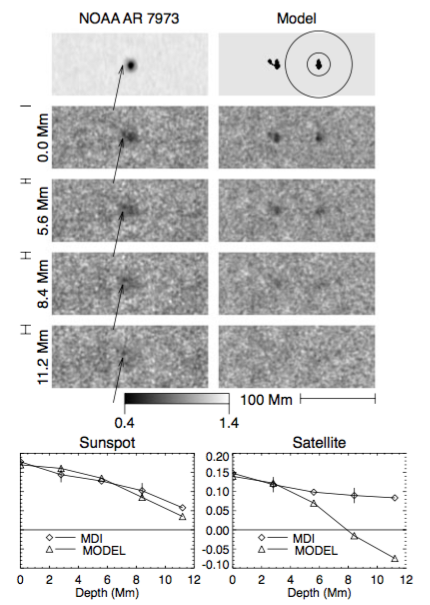
\includegraphics[width=0.95\textwidth]{fig_5.png}
        \end{figure}
    \end{columns}
\end{frame}

%-------------------------------------------------------------------%
\begin{comment}
\begin{frame}{Acoustic Modeling Based on Holographic Images}
    Flexible procedures, such as inversions, would characterize the
    acoustic environment in pysical terms such as:
    \begin{itemize}
        \item acoustic emissivity
        \item acoustic opacity
        \item refractivity
        \item flow velocity
    \end{itemize}
    where the last two result from the application of phase-sensitive
    holography
\end{frame}
\end{comment}
%-------------------------------------------------------------------%
\begin{comment}
\begin{frame}{Inversions (need more here)}
    Fredholm integral:
    $$ \langle|H_{+}(\mathbf{r},z)|^{2}\rangle =
    \int\textrm{d}^{2}\mathbf{r}'\int\textrm{d}z'g^{-1}
    (|\mathbf{r}-\mathbf{r}'|,z,z')S(\mathbf{r}',z') $$
    Source distribution:
    $$ S(\mathbf{r},z) = \int\textrm{d}^{2}\mathbf{r}'
        \int\textrm{d}z'g^{-1}(|\mathbf{r}-\mathbf{r}'|,z,z')
        \langle |H_{+}(\mathbf{r}',z')|^{2}  \rangle $$
\end{frame}
\end{comment}
%-------------------------------------------------------------------%
\begin{comment}
\begin{frame}{Phase-Sensitive Holography}
    Purpose is to incorporate the basic utilities of optical
    interferometry into solar interior diagnostics.
    The need for phase-sensitive holography is two-fold:
    \begin{enumerate}
        \item straight-forward quantitative probe of refractive anomalies
            that we expect from thermal perturbations
        \item Something else
    \end{enumerate}
    ``standard acoustic-power holography'' depends on anomalous sources
    and absorbers
\end{frame}
\end{comment}
%--------------------------------------------------------------------------%
\begin{frame}{Phase-Sensitive Holography}
{A \emph{gedanken} experiment}
    \vspace{-0.25cm}
    \begin{figure}
        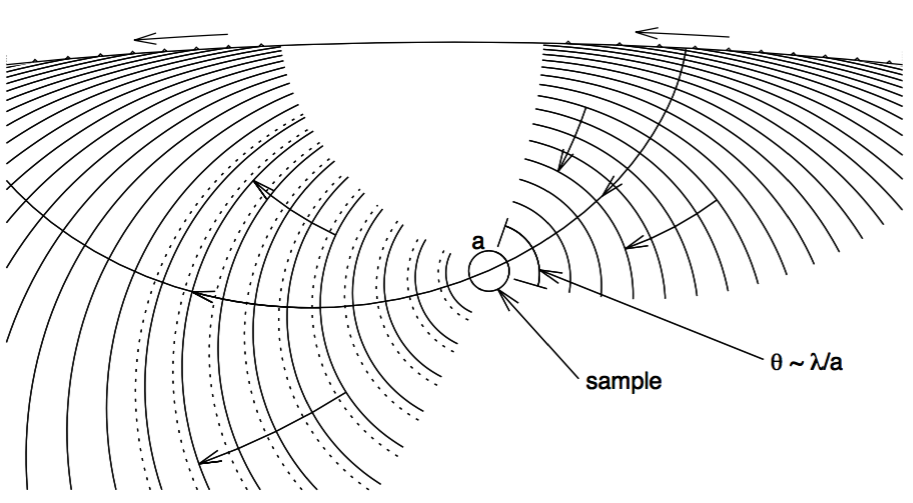
\includegraphics[width=\textwidth]{fig_6.png}
    \end{figure}
    \vspace{-0.25cm}
    \begin{itemize}
        \item Produce waves that travel from right to left, into the
            refractive sample.
        \item $a$ is the characteristic diameter of the sample.
    \end{itemize}
\end{frame}
%--------------------------------------------------------------------------%
\begin{frame}{Phase-Sensitive Holography}
{A \emph{gedanken} experiment}
    \begin{itemize}
        \item $\Delta{n} = 0$ $\rightarrow$ No phase-shift
        \item $\Delta{n} \neq 0$ $\rightarrow$ Phase-shift
            \begin{itemize}
                \item $\Delta{n} = \Delta{c_{s}}/c_{s} \rightarrow$
                    refractive perturbation
                \item $\Delta{t} \sim a\Delta{n}/c \rightarrow$
                    time delay
                \item $\Delta{\phi} \sim 2\pi\nu a\Delta{n}/c \rightarrow$
                    phase shift
            \end{itemize}
    \end{itemize}

    To relate $\Delta\phi$ to $H_{+}$ and $H_{-}$, define the
    \emph{temporal} Fourier transforms
    \begin{itemize}
        \item $ \check{H}_{+}(\mathbf{r},z,\nu)  $
            $ \leftrightarrow$
            $ {H}_{+}(\mathbf{r},z,t)  $
        \item $ \check{H}_{-}(\mathbf{r},z,\nu)  $
            $ \leftrightarrow$
            $ {H}_{-}(\mathbf{r},z,t)$.
    \end{itemize}
    Then
    $$ \Delta\phi = \arg\left(\left\langle
        \check{H}_{+}(\mathbf{r},z,\nu)
        \check{H}_{-}^{*}(\mathbf{r},z,\nu)
        \right\rangle
        _{\Delta\nu}
        \right) $$
\end{frame}
%--------------------------------------------------------------------------%
\begin{comment}
\begin{frame}{Correlations}
    Temporal correlation: $$
    C(\mathbf{r},z,\tau) = \int\textrm{d}t'H_{-}(z,\mathbf{r},t')
    H_{+}(z,\mathbf{r},t'+\tau) $$
    Extension of correlation for measuring horizontal flows: $$
    C(\mathbf{r},z,\mathbf{s},\tau) =
    \int\textrm{d}t'H_{-}(z,\mathbf{r},t')
    H_{+}(z,\mathbf{r}+\mathbf{s},t'+\tau) $$
    $$ \Delta\mathbf{r} = \mathbf{v}\Delta{t} = \mathbf{v}a\Delta{n}/c $$
    $$ \mathbf{U}(\mathbf{r},z) = \left\langle\check{H}_{-}^{*}
    (\mathbf{r},z,\nu)\nabla\check{H}_{+}(\mathbf{r},z,\nu)\right\rangle
    _{\Delta\nu} $$
\end{frame}
\end{comment}
%--------------------------------------------------------------------------%
\begin{frame}{Green's Functions}
    $$ G_{\pm}(|\mathbf{r}-\mathbf{r}'|,z,t-t') $$
    Characterizes the propagation of acoustic disturbances
    between a surface point,
    $(\mathbf{r}',0,t')$ and source point, $(\mathbf{r},z,t)$

    These propagations take place in the solar \emph{model}
    to which helioseismic observations, $\psi(\mathbf{r}',t')$.  are applied.
\end{frame}

\begin{frame}
    \Large\textcolor{lemon}{Computational seismic holography is
    intended as a braod and flexible diagnostic generality, not to be
    confined to any particular model.}
\end{frame}

\begin{frame}{Dispersionless acoustics}
    \begin{itemize}
        \item Pulse propagates in the form of an infintely thin \emph{wavefront}.
        \item $\mathbf{r}'$ responds with ripple characterized
            by the same infinitely sharp temporal profile as the
            source.
        \item The Green's function is invarient with
            respect to both time and horizontal translation.
    \end{itemize}
    $$ G_{+}(|\mathbf{r}-\mathbf{r}'|,z,t-t') =
    \delta\left(
    t-t'-\textcolor{mangotango}{T}\left(|\mathbf{r}-\mathbf{r}'|,z\right)\right)
       \textcolor{mangotango}{f}\left(|\mathbf{r}-\mathbf{r}'|,z\right)$$
       \begin{itemize}
           \item $T$: travel time
           \item $f$: amplitude of pulse
       \end{itemize}
\end{frame}

\begin{comment}
\begin{frame}{Dispersionless acoustics}
    $$ T(|\mathbf{r}-\mathbf{r}') = \int\limits_{{\Gamma}}\frac{\textrm{d}s}{c} $$
    $$ f^{2} = \frac{1}{4\pi{c}\cos\alpha}\frac{\sin\theta}{\sin\rho}
    \frac{\textrm{d}\theta}{\textrm{d}\rho} $$

    Acoustic energy flux density: $cf^{2}$
\end{frame}

\begin{frame}
    \begin{figure}
        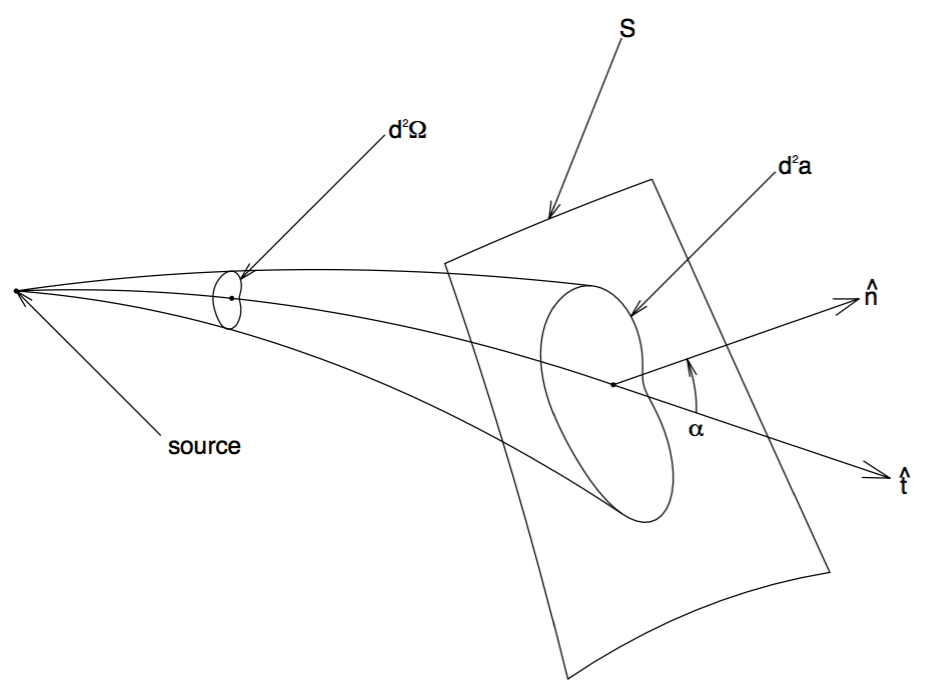
\includegraphics[width=\textwidth]{fig_7.png}
    \end{figure}
\end{frame}
\end{comment}

\begin{frame}{Dispersionless acoustics}{Reflected waves}
    \begin{itemize}
        \item $\nu>5.5$ mHz absorbed by photosphere.
        \item $\nu<4.5$ mHz reflected from photosphere.\\
            Green's function is characterized by a sum of $n$ components, where
            each $n$ is a ``skip'', or reflection from the photosphere.
    \end{itemize}
    \begin{enumerate}
        \item subjacent: $\rho$ decreases as $\theta$ increases
        \item superjacent: $\rho$ increases after reaching a minimum
            as $\theta$ continues to increase toward 180$^{\circ}$.
    \end{enumerate}
\end{frame}

\begin{frame}
    \begin{figure}
        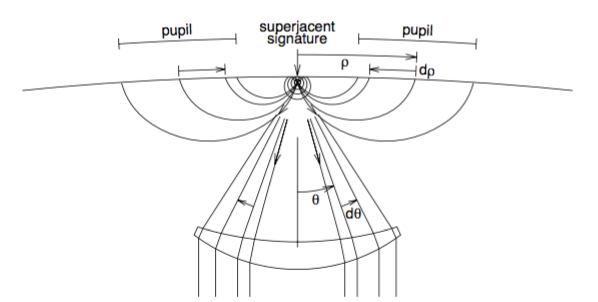
\includegraphics[width=\textwidth]{fig_4.png}
    \end{figure}
\end{frame}

\begin{frame}{Single-skip holography}
\begin{columns}
\column{0.30\textwidth}
T (travel time [s])\\
\vspace{1.5in}
f (amplitude)
\column{0.75\paperwidth}
    \begin{figure}
        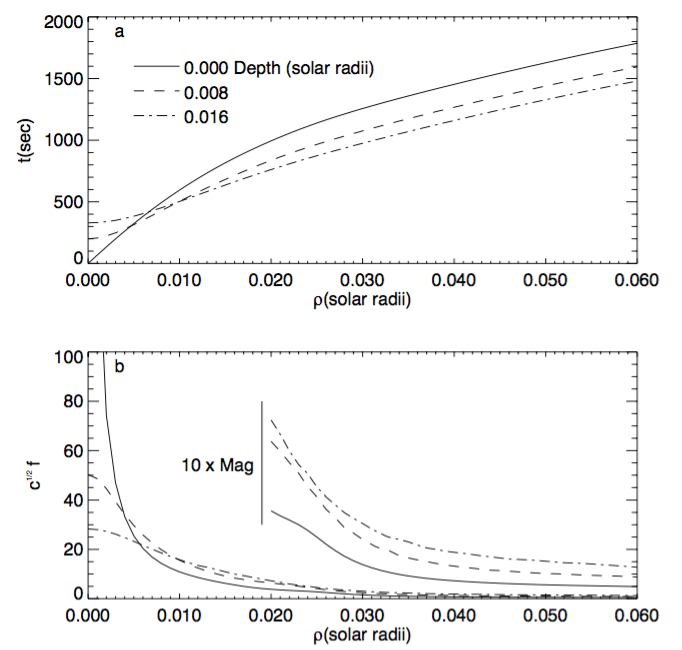
\includegraphics[width=0.8\textwidth]{fig_8.png}
    \end{figure}
\end{columns}
\end{frame}
\begin{frame}{Two-skip holography}
    \begin{figure}
        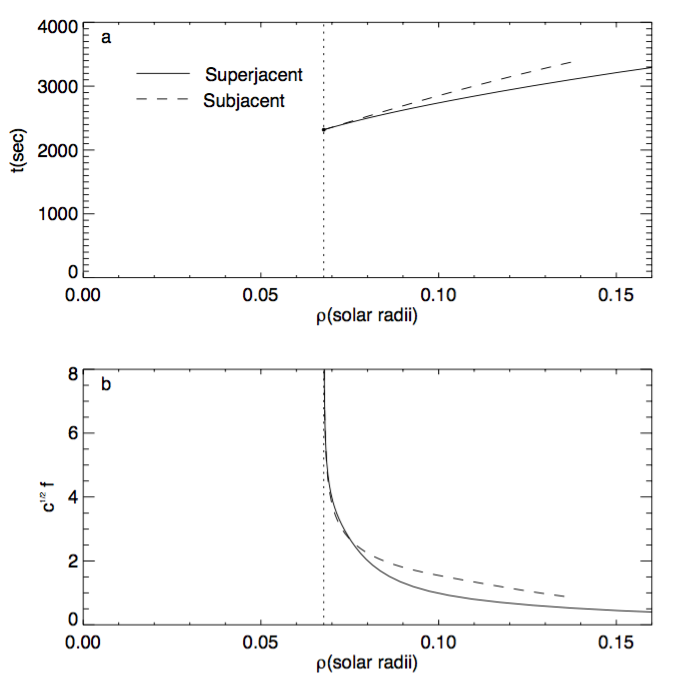
\includegraphics[width=0.7\textwidth]{fig_9.png}
    \end{figure}
\end{frame}

\begin{frame}
Phase correlation between dispersionless egression computation
$\check{H}_{+}$ and surface amplitude $\check{\psi}$
    \begin{figure}
        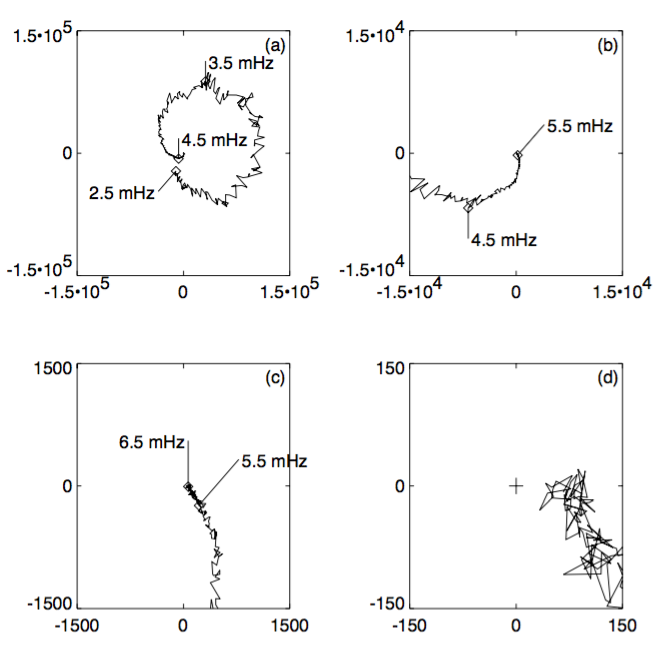
\includegraphics[width=0.8\textwidth]{fig_10.png}
    \end{figure}
\end{frame}

\begin{frame}
The phase of the correlation
    \begin{figure}
        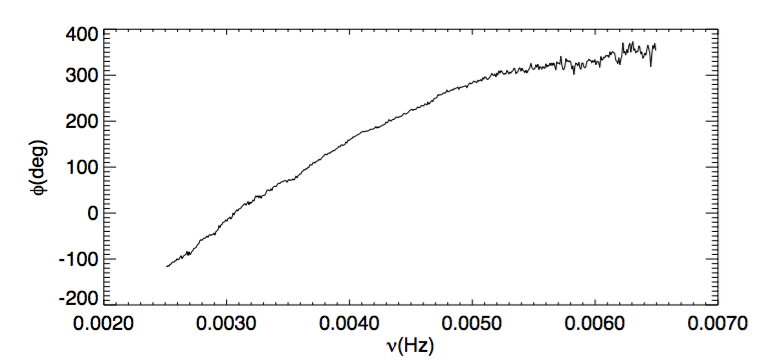
\includegraphics[width=\textwidth]{fig_11.png}
    \end{figure}
\end{frame}

\begin{frame}{Comparison to other techniques}
    \begin{itemize}
        \item time-distance helioseismology
            (aka.\ tomography)
        \item ring diagram analysis
    \end{itemize}
\end{frame}

%--------------------------------------------------------------%

\end{document}
